\documentclass[a4paper,12pt]{article}
\usepackage{amsmath,amssymb,amsfonts,amsthm}
\usepackage{tikz}
\usepackage [utf8x] {inputenc}
\usepackage [T2A] {fontenc} 
\usepackage[russian]{babel}
\usepackage{cmap} 
\usepackage{ gensymb }
% Так ссылки в PDF будут активны
\usepackage[unicode]{hyperref}
\usepackage{ textcomp }

% вы сможете вставлять картинки командой \includegraphics[width=0.7\textwidth]{ИМЯ ФАЙЛА}
% получается подключать, как минимум, файлы .pdf, .jpg, .png.
\usepackage{graphicx}
% Если вы хотите явно указать поля:
\usepackage[margin=1in]{geometry}
% Или если вы хотите задать поля менее явно (чем больше DIV, тем больше места под текст):
% \usepackage[DIV=10]{typearea}

\usepackage{fancyhdr}

\newcommand{\bbR}{\mathbb R}%теперь вместо длинной команды \mathbb R (множество вещественных чисел) можно писать короткую запись \bbR. Вместо \bbR вы можете вписать любую строчку букв, которая начинается с '\'.
\newcommand{\eps}{\varepsilon}
\newcommand{\bbN}{\mathbb N}
\newcommand{\dif}{\mathrm{d}}

\newtheorem{Def}{Определение}


\pagestyle{fancy}
\makeatletter % сделать "@" "буквой", а не "спецсимволом" - можно использовать "служебные" команды, содержащие @ в названии
\fancyhead[L]{\footnotesize Оптика}%Это будет написано вверху страницы слева
\fancyhead[R]{\footnotesize ФМХФ МФТИ}
\fancyfoot[L]{\footnotesize \@author}%имя автора будет написано внизу страницы слева
\fancyfoot[R]{\thepage}%номер страницы —- внизу справа
\fancyfoot[C]{}%по центру внизу страницы пусто

\renewcommand{\maketitle}{%
	\noindent{\bfseries\scshape\large\@title\ \mdseries\upshape}\par
	\noindent {\large\itshape\@author}
	\vskip 2ex}
\makeatother
\def\dd#1#2{\frac{\partial#1}{\partial#2}}


\title{4.3.5 \\ Изучение голограммы}
\author{Егор Берсенев} 
\date{9 февраля 2017 г.}

\begin{document}
	\maketitle
	\section{Цель работы}
		Знакомство с настройкой и работой гониометра, определение спектральных характеристик амплитудной решетки.
	\section{Оборудование}
		He-Ne-лазер, голограммы, набор линз, предметная шкала, экран, линейка.
	
	\section{Теоретическое введение}

	Осветим предмет когерентным источником. Пусть волна, отраженная предметом, создает в плоскости $z=0$ поле $F_s(x,y)=A(x,y)e^{i\phi(x,y)}$. Очевидно, что если мы в отсутствии предмета создадим поле $G$, которое удовлетворяет волновому уравнению и граничному условию $G(x,y,z)|_{z=0}=F_s(x,y)$, то мы получим поле, тождественное реальному.

	Теперь нужно описать реализацию на практике. Одной из первых идей является попробовать использовать фотопластинку. Но проблема заключается в том, что пластинка чувствительна лишь к интенсивности поля, т.е. к квадрату величины $F_s$. Это означает, что мы теряем информацию о фазе поля $F_s$. Проблема решается, если в добавок к волне, идущей от предмета, добавить известную волну (\emph{опорную}). Тогда волна от предмета будет интерферировать с опорной волной, что позволит сохранить информацию о фазе $F_s$.

	Итак, на пластинку падают теперь две волны $F_s$ и $F_0$, тогда

	\begin{equation}
		I=|F_s+F_0|^2
	\end{equation}

Положим, что ''прозрачность'' пластинки пропорциональна интенсивности света при записи, т.е. $T\sim I$. Тогда мы можем записать

\begin{equation*}
	T=|F_s|^2+|F_0|^2+F_sF_0^*+F_s^*F_0
\end{equation*}

Внимание нужно обратить на третье слагаемое: оно линейно по $F_s$, значит содержит всю информацию об амплитуде и, самое главное, о фазе волны предмета.

Фотопластинка, на которую описанным выше образом ''записывают'' изображение предмета, называется \emph{голограммой}.

Далее, подробнее опишем голограмму точечного источника. Пусть фотопластинка находится в плоскости $xy$ и на нее падает волна, исходящая из источника на расстоянии $d$ от голограммы. Это так называемая предметная волна и

\begin{equation}
	E_{\mathrm{obj}}=A(r)e^{-i\left( \sqrt{r^2+d^2}+\phi\right) },
\end{equation}

где $k=2\pi/\lambda$, $r^2=x^2+y^2$, $\phi$ -- начальная фаза. На небольших расстояниях можно считать $A(r)\approx A_0=\mathrm{const}$. А вблизи пучка $r\ll d$ и поэтому

\begin{equation}
	k\sqrt{r^2+d^2}\approx kd+\frac{kr^2}{2d}
\end{equation}

Этот переход называется \emph{приближением Френеля}. Тогда для предметного поля

\begin{equation}
	E(r)=A(r)e^{-i\left(kr^2/2d+\psi \right) }
\end{equation}

Очевидно, что если рассматривать волну, которая сходится где-то за голограммой, то ее поле $E'$ отличается лишь знаком в экспоненте. 

В качестве опорной волны выбираем плоскую волну с фазовым портретом, параллельных плоскости голограммы и тогда $E_{\mathrm{sup}}=A_{\sup}$.

Интенсивность, как мы видели раньше

\begin{eqnarray}
	I(r)=A_{\sup}^2+A_{\mathrm{obj}}^2+E_{\mathrm{obj}}A^*_{\sup}+E^*_{\mathrm{obj}}A_{\sup}
\end{eqnarray}

А для функции прозрачности имеем

\begin{equation}
	T(r)\sim A_{\sup}^2+A_{\mathrm{obj}}^2+2A_{\mathrm{obj}}A_{\sup}\cos\left(\frac{kr^2}{2d}+\theta\right),
\end{equation}

где $\theta$ -- некоторая постоянная фаза.  Из последней формулы следует, что (если пренебречь фазой) прозрачность максимальная при $r_n=\sqrt{2n\lambda d}$ и минимальна при $r_{2n+1}=\sqrt{(2n+1)}\lambda d$. Таким образом, голограмма точечного источника подобна зонной пластинке.

	\section{Ход работы}
		Перед началом работы настроим установку. Для этого включим лазер и осветим им шкалу. На удаленном экране получим дифракционную картину созданную крестообразной шкалой. Определим $\Delta x = 0.54\pm0.1 \,\text{см}$. Расстояние от образца до экрана равно $D = 114\pm 0.5,\text{см}$.
		
		\begin{equation}
		\frac{\lambda}{D}=\frac{\delta x}{L}\rightarrow D=\frac{\lambda L}{\delta x}=(1.14\pm 0.2)\cdot 10^{-2} \ \mbox{см}
		\end{equation}
		
		Теперь рассчитаем ту же величину с использованием линзы $f = 4\,\text{см}$. Расстояние от экрана до линзы $L_1 = 110\pm 1\,\text{см}$. Получим отсюда:
		
		\begin{equation}
		\Gamma=27.4\pm 0.3; \quad D_{\Gamma}=0.25\pm 0.1 \ \mbox{см}
		\end{equation}
		
		
		Теперь оценим расстояние от точечного источника до голограммы. Для этого получим контрастное изображение колец. Отметим радиусы нескольких светлых колец.
		
		\begin{table}[h!]
			\centering
			\caption{Радиусы темных колец}
			\label{my-label}
			\begin{tabular}{|l|l|l|l|l|l|}
				\hline
				n & 1   & 2 & 3   & 4   & 5 \\ \hline
				d, mm & 2.5 & 4 & 5.5 & 6.7 & 8 \\ \hline
			\end{tabular}
		\end{table}
		
		\newpage
		
		Построим график:
		
		\begin{center}
			\begin{figure}[h]
				\centering
				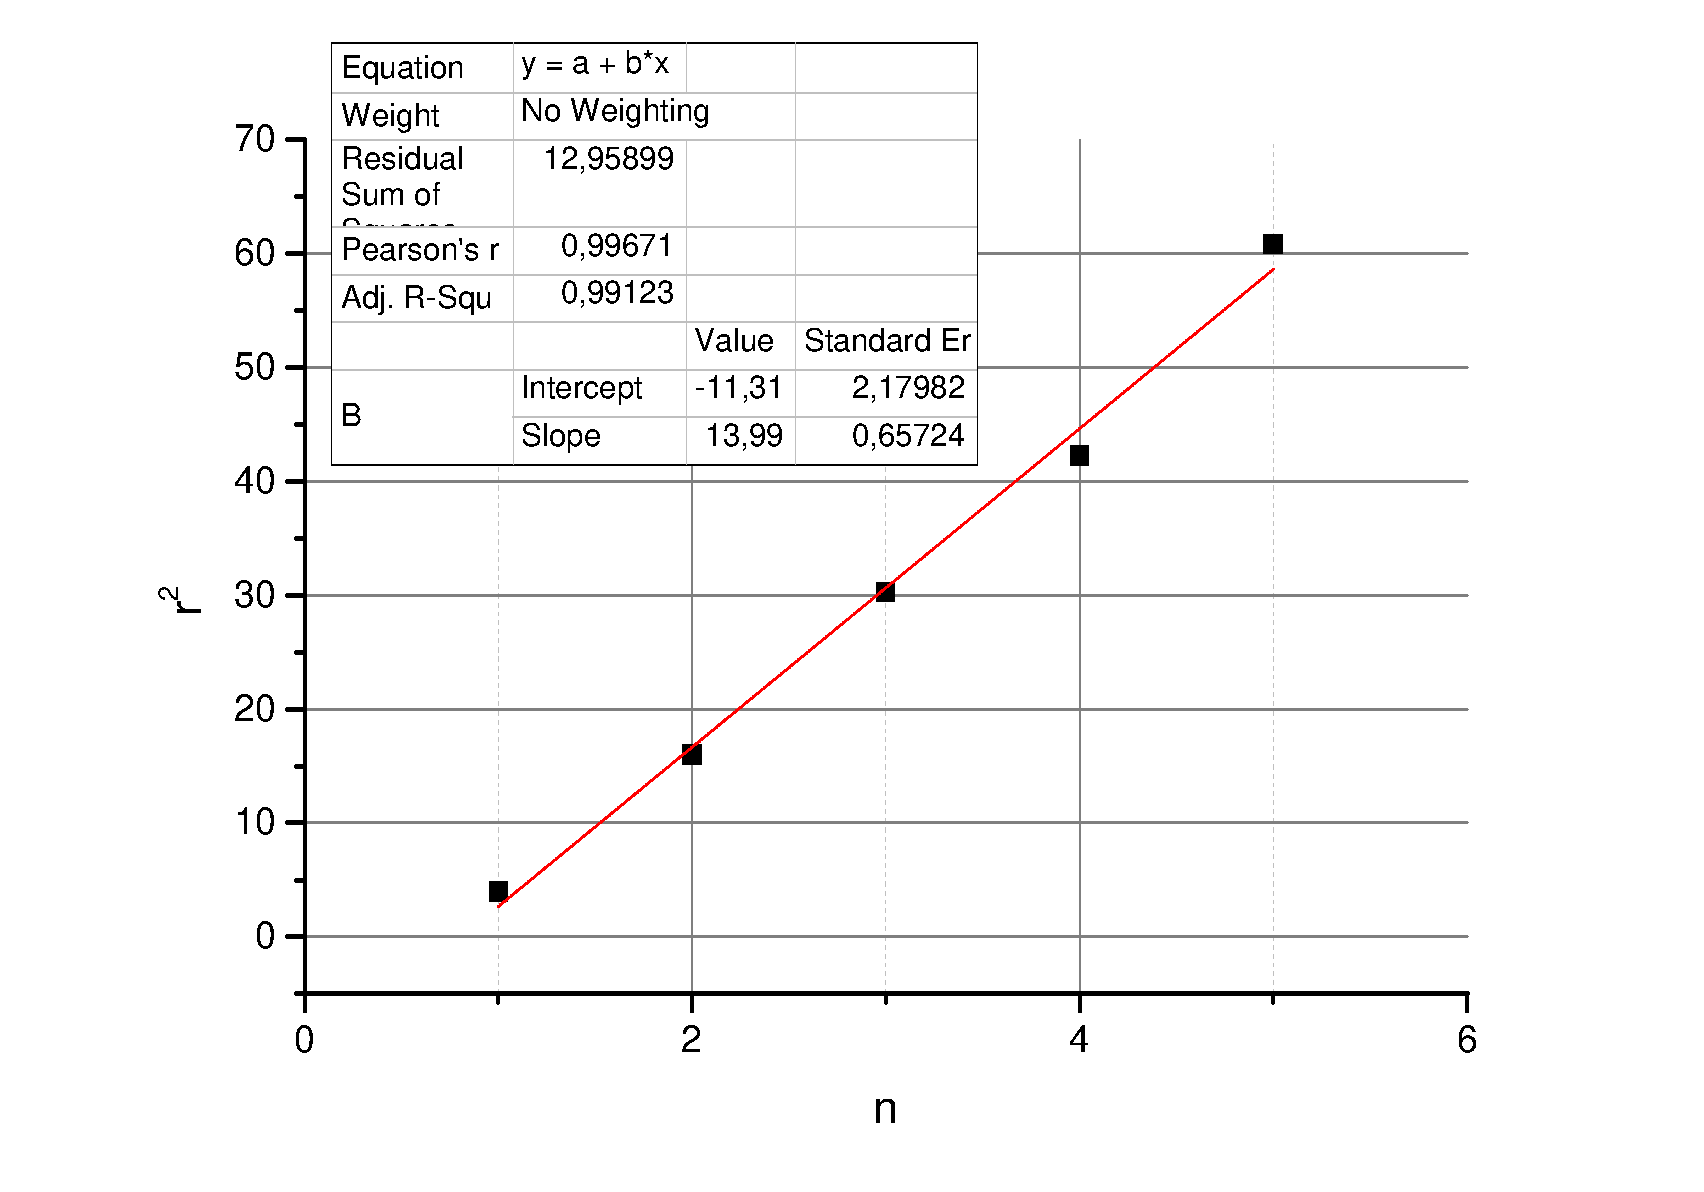
\includegraphics[width=0.6\linewidth]{graph}
				\caption{Зависимость $r^2=f(n)$}
				\label{fig:Graph1}
			\end{figure}
		\end{center}
		
		По формуле 
		\begin{equation}
			d = \frac{r_n^2}{2n\lambda \Gamma^2}
		\end{equation}
		
		Получаем $d = 20.2 \pm 1.4\,\text{мм}$
		
		Проделаем то же самое с помощью линзы с фокусным расстоянием $f = 4\,\text{см}$. Пусть $y = a - x$.
		
		\begin{equation}
		\frac{1}{f}=\frac{1}{x}+\frac{1}{b}\rightarrow x=\frac{bF}{b-F}
		\end{equation}
		
		$$
		a = 4\,\text{см} \quad y_1 = 7.5\,\text{см}\quad y_2 = -6.7\,\text{см}
		$$
		
		Исследуем фокусное расстояние тонкой линзы. Расстояние от экрана до голограммы равно $L = 107\pm 1\,\text{см}$. $D' = 3\,\text{мм}$
		
		$$
		\frac{b}{a} = \frac{D}{D'} \implies a=\frac{Db}{D'} = 4\pm 0.4 \,\text{см}		
		$$
		
		Считая голограмму тонкой линзой, получаем:
		\begin{equation}
		\frac{1}{f}=\frac{1}{a}+\frac{1}{b}\implies f=\frac{ba}{a+b}=3.85\pm 0.4 \, \mbox{см}
		\end{equation}
		
		Теперь заменим зеленый лазер на красный с длиной волны $\lambda_r = 632.8\,\text{нм}$. В этом случае  $L = 107\pm 1\,\text{см}$. $D' = 2\,\text{мм}$. Аналогично получаем $f = 2.25 \pm 0.4\,  \mbox{см}$

		
		
		
	\section{Вывод}
		При исследовании голограммы были выявлены ее фокусирующие свойства. Также было обнаружено, что фокусное расстояние голограммы для разных длин волн разное. Также мы наблюдали голограмму линейки и штыря.
	
\end{document}


